% !TEX TS-program = xelatex
% !BIB TS-program = bibtex
\documentclass[12pt,letterpaper]{article}
\usepackage{style/dsc180reportstyle} % import dsc180reportstyle.sty
\usepackage{float} % for [H] figure placement

%%%%%%%%%%%%%%%%%%%%%%%%%%%%%%%%%%%%%%%%%%%%%%%%%%%%%%%%
%%%% Title and Authors
%%%%%%%%%%%%%%%%%%%%%%%%%%%%%%%%%%%%%%%%%%%%%%%%%%%%%%%%

\title{DSC Capstone Q1 Report}

\author{Jevan Chahal\\
  {\tt j2chahal@ucsd.edu} \\\And
  Hillary Change \\
  {\tt hic001@ucsd.edu} \\\And
  Kurumi Kaneko \\
  {\tt kskaneko@ucsd.edu} \\\And
  Kevin Wong \\
  {\tt kew024@ucsd.edu} \\\And
  Brian Duke \\
  {\tt brian.duke@prismdata.com} \\\And
  Kyle Nero \\
  {\tt kyle.nero@prismdata.com} \\}

\begin{document}
\maketitle

%%%%%%%%%%%%%%%%%%%%%%%%%%%%%%%%%%%%%%%%%%%%%%%%%%%%%%%%
%%%% Abstract and Links
%%%%%%%%%%%%%%%%%%%%%%%%%%%%%%%%%%%%%%%%%%%%%%%%%%%%%%%%

\begin{abstract}
    \textcolor{Black}{
    The process of capturing what makes a creditor trustworthy or not is especially vital within the confines of bank data, due to the guidelines and ethics of what makes this data usable. Although the quantity of the data is massive, there are only a few available features that are explicitly useful in the confines of machine learning, which calls into question how we should measure customer's trustworthiness towards their creditors. Our methodology details the process of refining bank data into categories using Natural Language Processing, assessing individual's income based on bank data alone, and also measuring their credit worthiness both accurately and efficiently. 
    }
\end{abstract}

\begin{center}
Code: \url{https://github.com/hillarychang/dsc180a-capstone}
\end{center}

\maketoc
\clearpage

%%%%%%%%%%%%%%%%%%%%%%%%%%%%%%%%%%%%%%%%%%%%%%%%%%%%%%%%
%%%% Main Contents
%%%%%%%%%%%%%%%%%%%%%%%%%%%%%%%%%%%%%%%%%%%%%%%%%%%%%%%%

\section{Introduction}
Predicting a customer’s creditworthiness is an essential task for banks, as it informs decisions relating to the profitability and risks of loans, credit cards, and other financial services. While traditional credit scores are widely used, they often overlook important aspects of customer behavior, especially for individuals with limited credit history. We aim to develop an alternative approach by analyzing transaction data to create a new creditworthiness measure, which we will call the "Blank Score." By examining patterns in spending, income consistency, and transaction types, we hope to create a model that more accurately reflects individual financial reliability.

\subsection{Data Description}
The dataset, provided by Prism Data, consists of detailed transaction records that include fields such as \texttt{memo}, \texttt{amount}, \texttt{date}, and \texttt{category}.
\begin{itemize}
    \item \textbf{\texttt{prism\_consumer\_id} (Quantitative):} Unique identifier for each consumer, used to analyze spending and income patterns per user.
    \item \textbf{\texttt{prism\_account\_id} (Qualitative):} Identifier for each account, distinguishing multiple accounts for a single consumer or across consumers.
    \item \textbf{\texttt{memo} (Qualitative):} Descriptive text providing transaction details, such as "grocery store" or "ATM withdrawal," useful for categorization.
    \item \textbf{\texttt{amount} (Quantitative):} Transaction value, where positive values represent inflows (e.g., deposits) and negative values represent outflows (e.g., payments).
    \item \textbf{\texttt{posted\_date} (Qualitative):} Date each transaction was posted, enabling temporal analysis of spending trends.
    \item \textbf{\texttt{category} (Qualitative):} Pre-assigned transaction type label, such as "food" or "utilities," serving as a basis for categorization.
\end{itemize}

\section{Exploratory Data Analysis}
We first conducted Exploratory Data Analysis using transaction data given to us from our industry partner, Prism Data. This analysis allowed us to identify different patterns. In specific, we observed notable differences in spending behaviors across various time periods. For instance, we noticed that most purchases occurred on weekdays, while weekends had significantly less purchasing priority, suggesting that consumers prioritize certain purchases during the week. 

We also examined seasonal patterns within the dataset, which spans from 2020 to 2023. Certain months, like April and May, showed increased inflows likely due to tax returns, while December exhibited higher spending, likely due to holiday-related expenses. These patterns indicate regular income and expenditure behaviors that could be relevant for predicting creditworthiness.

\begin{figure}[H]
    \centering
    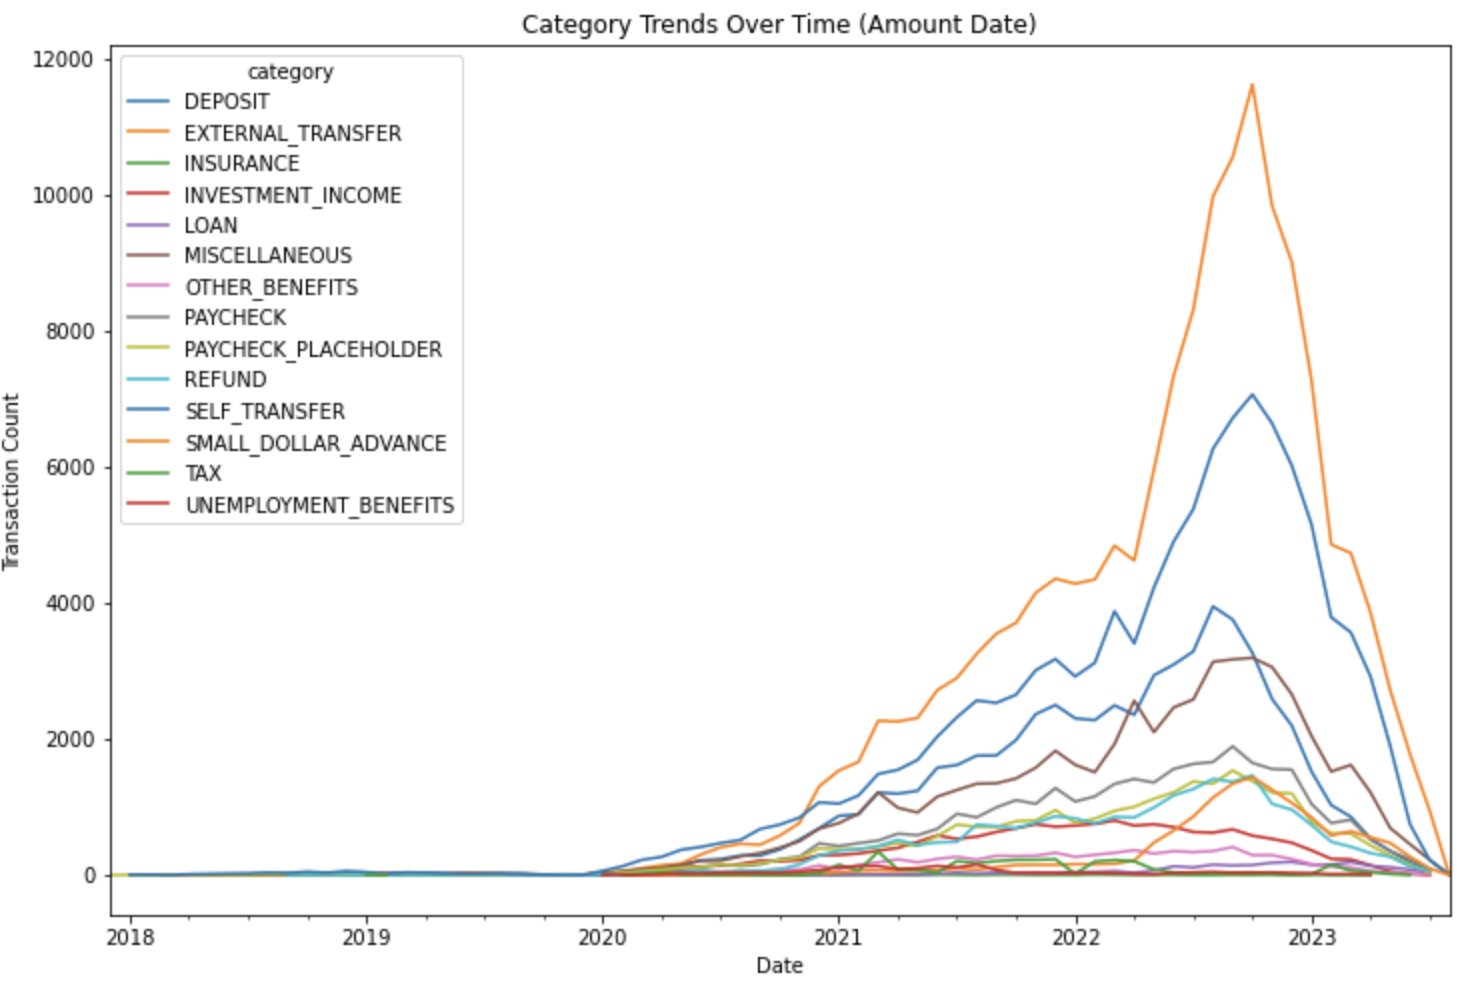
\includegraphics[width=\textwidth]{figure/category_time.png}
    \caption{Trends of transaction categories over time. This exploratory analysis visualizes patterns in transaction volume across different categories, revealing insights such as seasonal spending behavior and category-specific peaks. For example, categories like \texttt{DEPOSIT} and \texttt{EXTERNAL\_TRANSFER} show higher transaction counts in certain months.}
    \label{fig:category_trends}
\end{figure}

\begin{figure}[H]
    \centering
    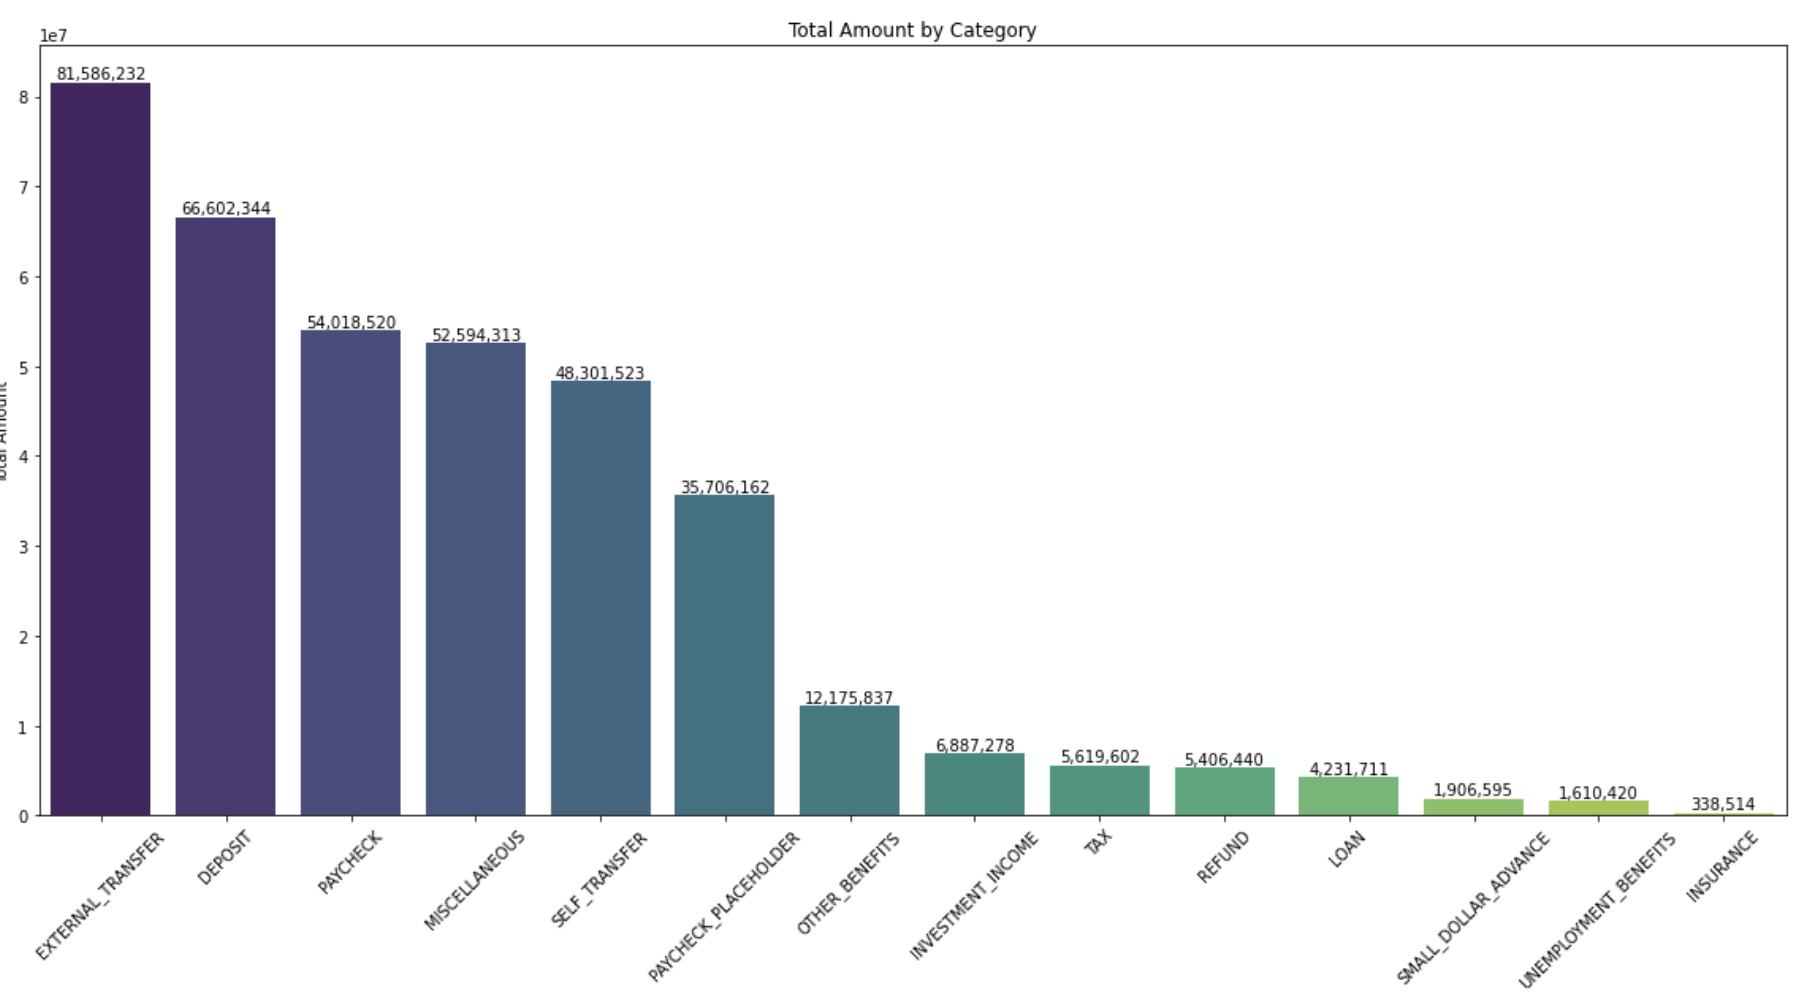
\includegraphics[width=\textwidth]{figure/amt_category.png}
    \caption{Bar chart showing the total amount spent across categories. This visualization highlights which categories contribute the most to overall expenditure, with \texttt{EXTERNAL\_TRANSFER}, \texttt{DEPOSIT}, and \texttt{PAYCHECK} as leading contributors. This information is valuable for understanding the primary financial activities within the dataset.}
    \label{fig:total_amount_by_category}
\end{figure}

\section{Train Test Split}

\begin{figure}[H]
    \centering
    \includegraphics[width=\textwidth]{figure/train_test_split1.png}
    \caption{Histogram of posted dates for the Inflow dataset. The distribution between training and testing sets is almost identical, indicating that the split was performed evenly across time periods. This ensures that both sets are representative of the overall data distribution and reduces potential biases when developing models.}
    \label{fig:inflow_date_distribution}
\end{figure}

\begin{figure}[H]
    \centering
    \includegraphics[width=\textwidth]{figure/train_test_split2.png}
    \caption{Histogram of posted dates for the Outflow dataset. Similar to the Inflow dataset, the distribution of dates is balanced between the training and testing sets, verifying an even temporal split. This helps in maintaining consistency and prevents temporal biases in model training and evaluation.}
    \label{fig:outflow_date_distribution}
\end{figure}

\section{Data Cleaning}

\begin{figure}[H]
    \centering
    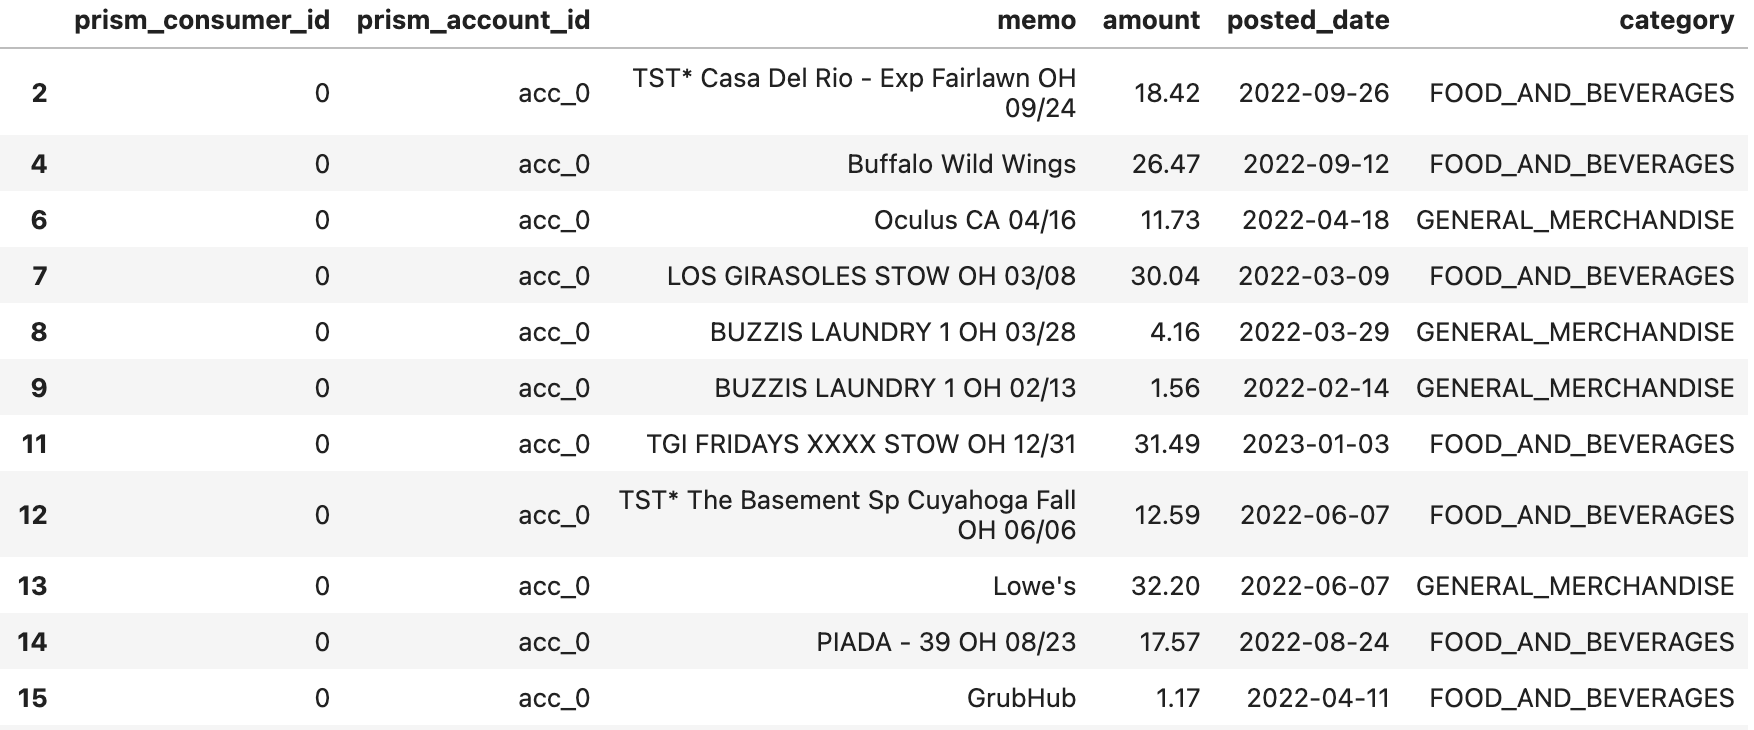
\includegraphics[width=\textwidth]{figure/nonclean_df.png}
    \caption{This table shows the memo dataframe before cleaning. Variations in text format, inconsistent capitalization, and extraneous characters can be observed, which motivated the cleaning process to improve uniformity in transaction descriptions.}
    \label{fig:pre_cleaned_memo}
\end{figure}

\begin{figure}[H]
    \centering
    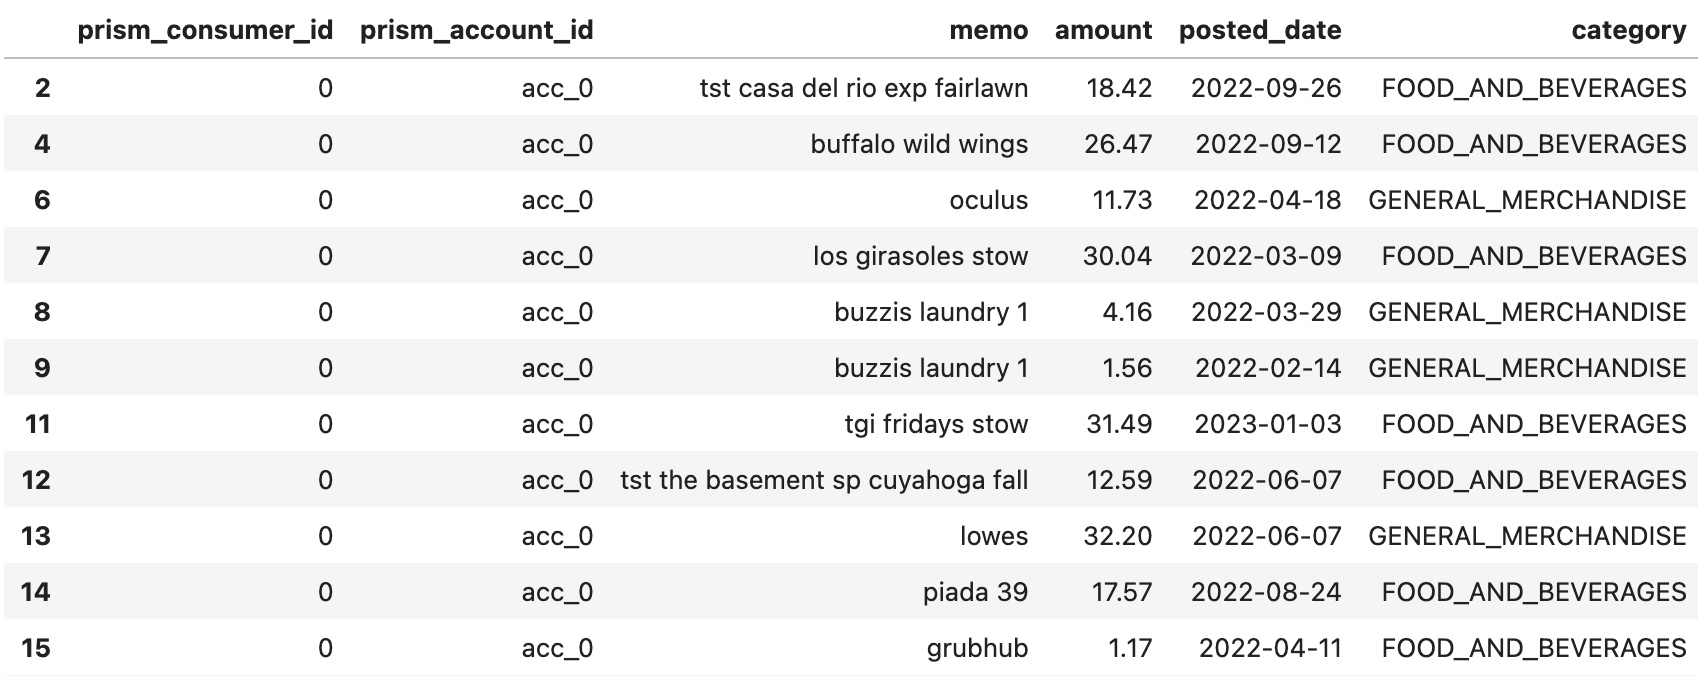
\includegraphics[width=\textwidth]{figure/clean_df.jpeg}
    \caption{This table represents the cleaned memo dataframe, where text preprocessing has been applied to ensure consistency across transaction descriptions. By converting to lowercase, removing punctuation, and standardizing certain tokens, the data is prepared for more accurate feature extraction and analysis.}
    \label{fig:clean_memo}
\end{figure}

\section{Methods}
\subsection{Data Cleaning}
To prepare the memo field for analysis, we first applied a series of cleaning steps to standardize the text. We transformed all text to lowercase for uniformity, removed any extraneous punctuation and symbols, and stripped out dates, state abbreviations, and recurring text that didn’t contribute to transaction categorization (ex., “POS withdrawal”). We also removed placeholder values, such as multiple X’s.

To prepare the dataset for modeling, we began by reviewing a sample of unique transaction memos from each category. This step provided insights into common patterns and inconsistencies, helping us determine the scope and focus of our cleaning tasks.

We then applied several transformations to standardize the data and improve its interpretability:

\begin{enumerate}
    \item \textbf{Date Removal}: We used regular expressions (RegEx) to locate and remove dates across entries in the memo column, as they did not contribute to the model's predictive goals and added unnecessary complexity. We also removed any extraneous or ambiguous patterns (e.g., “XXXX” entries).

    \item \textbf{Pattern Recognition}: Specific patterns and keywords were identified as indicators of certain transaction categories. For example, "TST" reliably associated with "Food and Beverages," while strings like "APPLE.COM/BILL" were linked to "General Merchandise." We flagged these patterns to automate future classifications and reduce manual intervention.

    \item \textbf{Selective Character Retention}: To preserve potentially valuable information, we retained certain characters such as dots ('.'). This choice allowed us to keep URLs or email addresses within the memo field, which could provide clues to the transaction category.

    \item \textbf{Transaction Labels}: We also identified recurring phrases such as "POS Withdrawal," location-specific markers (e.g., “CA 10/27” for state and date), and labels indicating recurring payments. These were removed for as they did not contribute to the model's predictive goals and added unnecessary complexity.

    \item \textbf{Text Normalization}: All text was converted to lowercase to reduce variability due to case differences.
\end{enumerate}

By implementing these steps, we improved data consistency and ensured key transactional information was preserved, enhancing our model's ability to accurately predict customer creditworthiness.

\section{Feature Engineering}
We applied Term Frequency-Inverse Document Frequency (\texttt{TF-IDF}) to convert the text in the \texttt{memo} field into numerical features. By using unigrams and bigrams, we captured meaningful phrases like \texttt{ATM withdrawal} and \texttt{grocery store}. \texttt{TF-IDF} proved to be highly predictive, assisting in accurately identifying transaction types.

\textbf{Date and Amount Features:} We engineered additional features based on transaction dates and amounts:
\begin{itemize}
    \item For date features, we created variables such as \texttt{day\_of\_week} and \texttt{day\_of\_month}, adding a flag for the first day of each month.
    \item For amount features, we flagged transactions ending in \texttt{.00} (referred to as \texttt{A00}), which is commonly seen in ATM withdrawals. This pattern helped distinguish ATM transactions from other transaction types.
\end{itemize}

\section{Model Training}
\textbf{Logistic Regression:} We first trained a logistic regression model as a baseline.

\textbf{Random Forest:} To capture more complex interactions, we also trained a random forest model.

\section{Evaluation Metrics}
We evaluated our models using accuracy, precision, recall, and a 9x9 confusion matrix to assess categorization performance across different transaction types. 

\section{Results}
\subsection{Model Performance}
\textbf{Logistic Regression:} The logistic regression model

\textbf{Random Forest:} The random forest model

\subsection{Confusion Matrix and Category-Specific Metrics}
The confusion matrix revealed that the random forest model accurately classified high-frequency categories but displayed some overlap in rarer ones.

\subsection{Precision and Recall by Category}
TF-IDF features were the main indicators for categorization, particularly in identifying terms within the \texttt{memo} field. Date and amount features provided additional value for regular and specific transaction types, such as rent payments and ATM withdrawals.

%%%%%%%%%%%%%%%%%%%%%%%%%%%%%%%%%%%%%%%%%%%%%%%%%%%%%%%%
%%%% Reference / Bibliography
%%%%%%%%%%%%%%%%%%%%%%%%%%%%%%%%%%%%%%%%%%%%%%%%%%%%%%%%

\bibliography{reference}
\bibliographystyle{style/dsc180bibstyle}

\end{document}
